

\documentclass[%
	final,
	narroweqnarray,
	notitlepage,
	inline,
	twoside,
	]{ieee}

\usepackage{tikz}
\usepackage{listings}\usepackage{subfigure}
\usetikzlibrary{calc,positioning,backgrounds,trees,automata}

\newcommand{\latexiie}{\LaTeX2{\Large$_\varepsilon$}}



\begin{document}

%----------------------------------------------------------------------
% Title Information, Abstract and Keywords
%		no ref, fig, tab
%		should stand alone
%----------------------------------------------------------------------

\begin{titlepage}

\newcommand{\HRule}{\rule{\linewidth}{0.5mm}} % Defines a new command for the horizontal lines, change thickness here

\center % Center everything on the page
 
%----------------------------------------------------------------------------------------
%	HEADING SECTIONS
%----------------------------------------------------------------------------------------

\textsc{\LARGE Rochester Institute of Technology}\\[1.5cm] % Name of your university/college
\textsc{\Large Department of Computer Science}\\[0.5cm] % Major heading such as course name
\textsc{\large Advanced Computer Vision}\\[2cm] % Minor heading such as course title

%----------------------------------------------------------------------------------------
%	TITLE SECTION
%----------------------------------------------------------------------------------------

\HRule \\[0.4cm]
{ \huge \bfseries Natural Scene Classification\\
\bigskip
Final Report}\\[0.7cm] % Title of your document
\HRule \\[1.5cm]

\begin{minipage}{0.8\textwidth}
\begin{flushleft} \large
\emph{Authors:}\\
Karina \textsc{Damico} \\
Pauline \textsc{Martial} % Your name
\end{flushleft}
\end{minipage}

\begin{minipage}{0.8\textwidth}
\begin{flushright} \large
\emph{Supervisor:} \\
Dr. Roger \textsc{Gaborski} % Supervisor's Name
\end{flushright}
\end{minipage}\\[5cm]

{\large February 14, 2013}\\[3cm] 
\vfill % Fill the rest of the page with whitespace
\end{titlepage}              
\nopagebreak
\tableofcontents
\newpage

\begin{abstract}
Scene categorization is a fundamental problem in image understanding. It is a challenging task in computer vision and widely applied in many fields, such as image retrieval, video surveillance, travel navigation or medical browser. Large image collections such as the Internet require efficient organization which is why a lot of attempts were performed to design automated systems to solve scene classification task in recent years.\\
The study presented in this paper aims to obtain high accuracy of scene classification through creating an advanced feature vector based on multiple feature sets extracted using Gabor filters, \textsc{CENTRIST} and color histograms. The goal is to produce feature vectors that describe the scene as accurately as possible. Each feature extraction method is first examined alone, then is combined with features obtained with other methods and tested on accuracy improvement. This paper shows the high performance obtained when combining these techniques. \\

\end{abstract}

%----------------------------------------------------------------------
% SECTION I: Introduction
%----------------------------------------------------------------------

    
\section{Introduction}
\label{sec:Introduction}

\PARstart  Scene classification is different from conventional object detection. The scene is a unique composition of several objects related and organized in often unpredictable layout. The relationships between objects and their organization mostly define the scene class. It makes classification task even more difficult, as a computer is unable to "understand" such relationships. Object-based judgement is able to provide more or less satisfactory results for man-made scenes as the object functional representation may itself supply sufficient information for labelling a scene. The situation is much more complicated for classifying natural scenes, where separate object detection does not provide enough information to relate the image to a particular category. High level features stay beyond any existing technique: semantic descriptors are not recognizable by computers. Thus, images have to be described by low level descriptors that aim to mimic semantic content of the image and make it understandable for computers.\\

In the study presented in this paper, each feature is investigated independently before being combined with other features. Features are evaluated using statistical methods as well as individual classification results. Statistical evidence is gathered primarily from the training set as inclusive or exclusive validation runs. This further provides insight into how representative is the feature for images of the same category. Classification results are generated from an exclusive subset of the training set as well as the test set.\\

The following of the paper is organized as follows. In section \ref{sec:approach}, our global approach chosen to solve scene recognition problem is explained. Sections \ref{sec:Gabor}, \ref{sec:CENTRIST} and \ref{sec:Color} respectively detail how Gabor, \textsc{Centrist} and color histogram feature descriptors are defined and used to describe the image. Obtained feature vectors are combined in section \ref{sec:Hybrid} and their performance is evaluated. Section \ref{sec:Conclusion} concludes this paper and summarizes the best results obtained. 
%----------------------------------------------------------------------
% SECTION II: Overview of the approach
%----------------------------------------------------------------------
\section{Overview of the Approach}
\label{sec:approach}
In order to have a scene classification as accurate as possible, several methods are used and combined. This choice was made with the assumption that because methods have their best efficiency for different classes, combining them should improve the overall accuracy. Results presented in section \ref{sec:Hybrid} further revealed that this assumption was true. \\
The chosen methods for scene classification are Gabor descriptors (described in section \ref{sec:Gabor}), \textsc{Centrist} feature vectors (described in section \ref{sec:CENTRIST}) and color histogram feature vectors (described in section \ref{sec:Color}). Those three descriptors are very different and use complementary information of the images. This is the key that enable an efficient combination of the feature vectors. 


%----------------------------------------------------------------------
% SECTION III: Gabor-GIST descriptor
%----------------------------------------------------------------------
\section{Gabor-\textsc{Gist} Descriptor}
\label{sec:Gabor}
Gabor descriptors proved their efficiency as robust texture descriptors. Similarity between low level processing in biological vision and Gabor filter banks was found and proved by Daugman~\cite{daugman}. Thus, Gabor descriptor is the way to make computer "understand" images in the way human brain does it.

The Gabor feature extraction consists of designing a set of Gabor filters in the spatio-frequency domain, and  forming a bank of filters to be applied to the images in order to transform information from the pixel space into the feature space. In the spatial domain, a 2D Gabor filter is a Gaussian kernel function modulated by a sinusoidal plane wave. The Gabor filters are self-similar: all filters can be generated from one mother wavelet by dilation and rotation~\cite{bib:Gist4}.

In this study, all the experiments were conducted with single 12 filter Gabor bank, but different techniques to preprocess data and reduce dimensionality were used.
\subsection{Gabor Bank Formation}
\label{subsec:Gab_Bank}
Gabor descriptor for an image is computed by passing the image through the Gabor filter bank. Gabor filter is a linear band-pass filter whose impulse response is defined as a Gaussian function modulated with a complex sinusoid.
Mathematically, a Gabor filter of a particular orientation and frequency is a sinusoid modulated by a Gaussian:
 \begin{displaymath}
h(x,y) = s(x,y)g(x,y)
\end{displaymath}
where $s(x, y)$ is a sinusoidal plane and $g(x, y)$ is a 2-D Gaussian. The Gaussian is represented by:
\begin{displaymath}
g(x,y) = \frac{1}{{\sqrt{2\pi\sigma}}}e^{-1/2(\frac{x^2}{\sigma_x^2} + \frac{y^2}{\sigma_y^2})}
\end{displaymath}
and $s(x,y)$ as:

\begin{displaymath}
s(x,y) = e^{-j2\pi(u_0x + v_0y)}
\end{displaymath}
The filter has a real and an imaginary component representing orthogonal directions. The two components may be formed into a complex number or used individually~\cite{bib:Gist2}.\\

A Gabor filter in 2 dimensions can be used to approximate the frequency and spatial response of the different scene categories.
Gabor filters can be viewed as specific edge detectors, which are able to percept edges of a certain orientation and strength.
A filter bank consisting of filters with 3 different scales (4, 8 and 16) and 4 orientations (0, 45, 90 and 135 degrees) was considered for feature extraction, giving a total of 12 Gabor filters bank. 

\subsection{Gabor Histogram Approach}
\label{subsec:Gab_hist}
The idea of this method is to calculate intensity histogram for Gabor filtered images. A color image converted into grayscale was split into four horizontal pieces in order to preserve some spatial information and potentially increase the classification accuracy. Each quarter of an image in the training and testing sets  was convolved with the filter bank. Intensity histogram was calculated from each piece of the image (32 bin histograms showed similar accuracy to 64 bins). Thus, the feature vector dimensionality is 1x128. 
Testing was performed in two ways:
\begin{itemize}
\item Calculating average histogram for each class from training images, and then comparing it  with histograms of testing images using Euclidian distance,
\item Using Multilayer Perceptron neural network. 
\end{itemize}

\begin{figure}
  \centering
    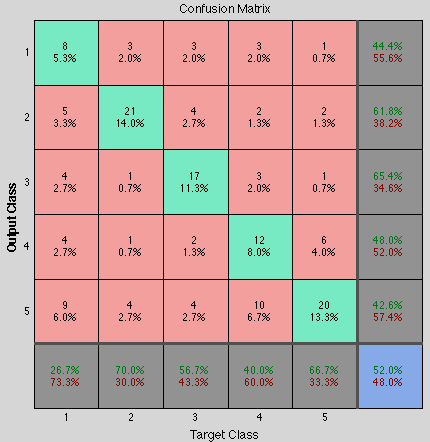
\includegraphics[width=0.4\textwidth]{table1}
  \caption{Confusion matrix for Gabor Histogram method 1-Coast; 2-Forest; 3-Highway; 4-Mountain; 5-Tall Building}
  \label{fig:table1}
\end{figure}

\noindent Both classification methods performed similarly with 52\% overall accuracy (see figure \ref{fig:table1}). Note that error rates differ from a category to another category. Because Gabor histogram approach performed very poorly, it was decided to continue experimenting with other approaches.

\subsection{Gabor "Manual-Bin" Histogram Approach}
\label{subsec:Gab_manhist}
As mentioned above, the histogram approach leads to the loss of the spatial information: it only indicates the strength of responses in certain directions and scales. The idea of "manual-bin" histogram approach is to calculate the value for each bin separately and thus save the response spatial information and intensity.

\begin{figure}
  \centering
    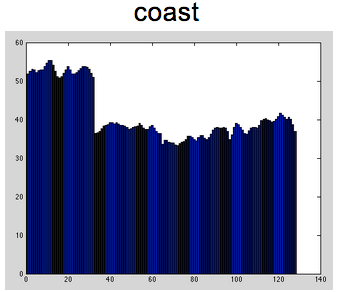
\includegraphics[width=0.4\textwidth]{Image1}
  \caption{Avaraged histogram for Coast category with Gabor "manual-bin" histogram approach}
  \label{fig:image1}
\end{figure}


The method was tested using MLP on 150 testing images and performed even worse than previous approach - misclassification rate of 51\%. Overall histogram dimensionality reduction approaches on grayscale images showed unsatisfactory classification accuracy, hence it was decided to leave histogram idea and move to Gabor-\textsc{Gist} descriptor.

\subsection{Gabor-\textsc{Gist} Visual Descriptor}
\label{subsec:Gab_GIST}

\subsubsection{Image Preprocessing}
\label{subsubsec:Gab_GISTpreproc}
Gabor-\textsc{Gist} feature extraction was performed on color image in contrast to previous approaches. Gabor filter bank (12 filters) was applied to each color plane of RGB images. For better results, color images were first preprocessed before being filtered: images were whitened and contrast was adjusted.

The purpose of whitening is removing pairwise, linear correlations, and thus remove noise and "simplify" an image. Whitening can be done through designing a filter in the frequency domain that will flatten the spectrum of a natural image. Amplitude spectrum of such filter has to rise linearly with frequency, to compensate for the amplitude spectrum of natural images. This can be done through defining a grid of frequency coordinates. Because convolution in the space domain is equivalent to multiplication in the frequency domain, whitening can be performed through multiplying the spectrum of the image with the spectrum of the filter and taking the inverse Fast Fourier Transform of the filtered image (see figure \ref{fig:image2_3}.b).
Contrast normalization is the standard operation to be done after whitening. For this project, normalization was done by dividing the output of the whitening step by the local luminance variance~\cite{bib:Gist2}~\cite{bib:Gist3}. 


\subsubsection{\textsc{Gist} Feature Extraction}
\label{subsubsec:Gab_GISTExtr}
In the scope of this project, \textsc{Gist} dimensionality was reduced using an averaging over non-overlapping square image blocks (for this project, fixed 4x4 grid of sub-regions over the map was considered)~\cite{bib:Gist1}. Thus, the size of feature vector is 1x576: 4x4 grid (16 windows where average values is computed) x 12 (filters in the Gabor bank) x 3 (number of color planes for RGB image).

\begin{figure}
  \centering
	\mbox{
	\subfigure{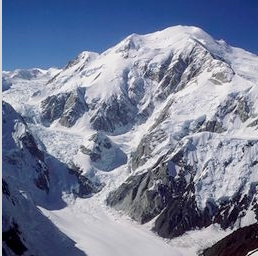
\includegraphics[width=0.25\textwidth]{Image2}
	\quad
	\subfigure{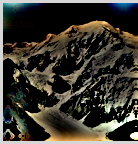
\includegraphics[width=0.25\textwidth]{Image3} }}}
  	\caption{a) Original Image and b) Whitened Image}
  	\label{fig:image2_3}
\end{figure}
\begin{figure}
  \centering
	\mbox{
	\subfigure{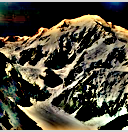
\includegraphics[width=0.25\textwidth]{Image4}
	\quad
	\subfigure{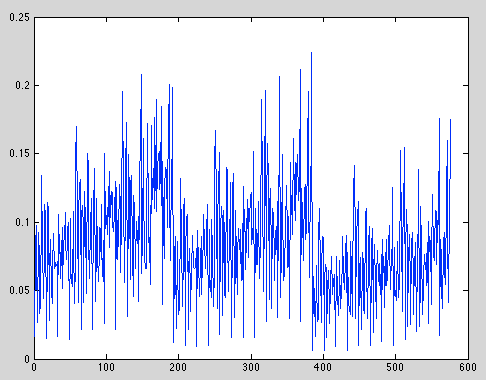
\includegraphics[width=0.25\textwidth]{Image5} }}}
  	\caption{a) Contrust Normalized Image and b) Gabor GIST visualization}
  	\label{fig:image4_5}
\end{figure}

\subsubsection{Classification Results}
\label{subsubsec:Gab_GISTres}
Similarly to previous approaches, MLP neural network with single hidden layer was considered as a classifier. All images form the training set were converted into 1x576x69 feature matrixes for each category (1x576 feature vector, 69 images in each category in the training set). Then training matrices were converted into input matrix 576x345. The corresponding target matrix has 5x345 for the training set and 5x150 for the testing set. Testing matrix size is 576x150 (testing set contains 150 images). Training set was divided into three categories: training (70\% of training images), validation (15\%) and testing (15\%). \\ The number of input neurons is equal to the number of features in the feature vector: 576. The number of hidden nodes was found experimentally and the value of 300 was the optimal number of hidden nodes. The number of outputs is the number of categories: 5 classes of scenes in the dataset.

Overall classification accuracy with Gabor-\textsc{Gist} features on 150 training set reached 86\%. Error rate differs from category to category, for example Forest images were classified correctly in 100\% of cases, when Highway had the lowest accuracy - only 70\% of correctly classified images. See confusion matrix in figure \ref{fig:table2} for more details.
\begin{figure}
  \centering
    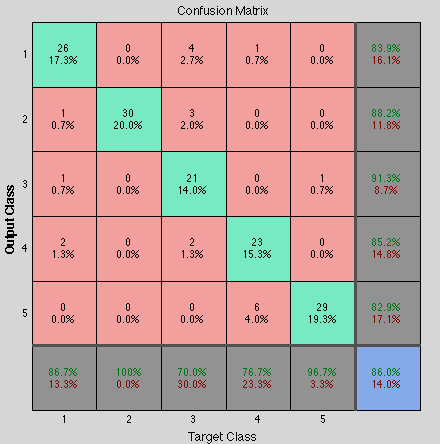
\includegraphics[width=0.4\textwidth]{Table2}
  \caption{Confusion matrix for Gabor-\textsc{Gist}. 1-Coast; 2-Forest; 3-Highway; 4-Mountain; 5-Tall Building}
  \label{fig:table2}
\end{figure}
Comparably to Gabor histogram approaches, Gabor-\textsc{Gist} over color image performed significantly better. Hence, Gabor-\textsc{Gist} features will be used for the hybrid feature vector creation.

%----------------------------------------------------------------------
% SECTION III: CENTRIST descriptor
%----------------------------------------------------------------------
\section{\textsc{Centrist} Descriptor}
\label{sec:CENTRIST}

\subsection{Computation of CT Value}
CENsus TRansform hISTogram (\textsc{Centrist}), is a visual descriptor used to identify scene categories~\cite{bib:centrist}. The \textsc{Centrist} feature vector is perfectly suitable for scene classification because this descriptor encodes the structural properties of a given image without keeping the detailed textural information that would not be helpful for this problem. \\
\begin{figure}
  \centering
    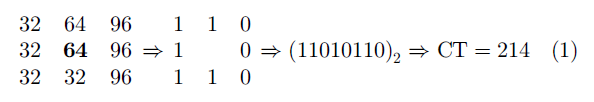
\includegraphics[width=0.5\textwidth]{CTvalueBasic}
  \caption{CT value calculation}
  \label{fig:CTvalueBasic}
\end{figure}
\begin{figure}
  \centering
    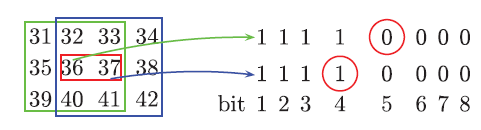
\includegraphics[width=0.5\textwidth]{CTvalueDependencies}
  \caption{CT value calculation for 2 adjacent pixels. Red circles reveal  dependencies between CT values: because $36<37$ when calculating CT value of green box center pixel, the relation will be $37>36$ when calculating CT value of blue box center pixel}
  \label{fig:CTvalueDependencies}
\end{figure}
The \textsc{Centrist} feature vector of a given image is calculated in 2 distinct steps:
\begin{enumerate}
\item First, the CT value for each pixel is computed. This is performed by a call to \textsc{Matlab} function \texttt{compare.m} for each pixel of the image. 
\item Once the CT values of all pixels of the image have been calculated, the histogram of the CT values is computed using function \texttt{CENTRIST4lines.m}. This histogram is the \textsc{Centrist} feature vector. 
\end{enumerate}
\medskip 
The CT value is calculated as follows: for each pixel, the 8 neighbours are compared to the center pixel value and are assigned value 0 if they are greater than the pixel value, 1 is they are smaller (see figure \ref{fig:CTvalueBasic}). Concatenating all 8 bits give a binary number with value between 0 and 255. This is the CT value. Figure \ref{fig:CTvalueDependencies} shows the obtained CT values for two adjacent pixels. It reveals dependencies between CT values: the right neighbour of a pixel for a given 3x3 pixels square will be the left neighbour for the adjacent 3x3 square. Thus if the right neighbour pixel value is greater (for example in figure \ref{fig:CTvalueDependencies}, $37>36$), then the left neighbour will be smaller for the next CT value computation ($36<37$).\\

\subsection{Parameters}
The \textsc{Matlab} function \texttt{CTfeatureVector.m} creates the feature vector \textsc{Centrist} for all training and testing images and saves data in a \texttt{.mat} file. In order to obtain the best performance, different parameters have to be tested. The following parameters have been used for the rest of the project since they produced the smallest misclassification rate:
\begin{itemize}
\item Downsizing the image to a ratio of 0.125. This reduces the computation time and keeps the relevant information of the image.
\item Dividing the image into 4 lines seemed to be the most efficient: instead of considering the image as a whole entity, it is divided into 4 lines. The \textsc{Centrist} vector is computed for each line and the 4 \textsc{Centrist} vectors are concatenated to obtain the \textsc{Centrist} vector of the image. This enable to keep some of the spatial information in the image that can help classifying scenes.
\item Histogram Intersection Method. In order to compare the \textsc{Centrist} feature vector of a tested image to the mean of the \textsc{Centrist} vectors of images belonging to a given class, the measure of difference must be calculated. This can be done using the Euclidian distance or the Histogram Intersection Method. The Histogram Intersection Method generated much better classification than when using the Euclidian distance. 
\item 40 bins are used for the histograms. This is the best compromise between the classification rate, the computation time and the size of the generated \textsc{Centrist} feature vector. 
\end{itemize}

\subsection{Results with a Neural Network}
When fed into a neural network, the \textsc{Centrist} method gives a misclassification rate of 14\% (see figure \ref{fig:table3}) which is a correct value for a single classification method. Note that even if the overall misclassification rates for Gabor-\textsc{Gist} (figure \ref{fig:table2}) and for \textsc{Centrist} (figure \ref{fig:table3}) are both 14\%, the misclassification rates vary for each category. This means that the method used will affect each categorie's misclassification rate. For example the Tall Building category has a misclassification rate of 0\% with the \textsc{Centrist} descriptor and 3.3\% with Gabor-\textsc{Gist}. At the opposite, the Coast category is much better classified if Gabor-\textsc{Gist} is used (13.3\% instead of 23.3\% with \textsc{Centrist}). 
\begin{figure}
  \centering
    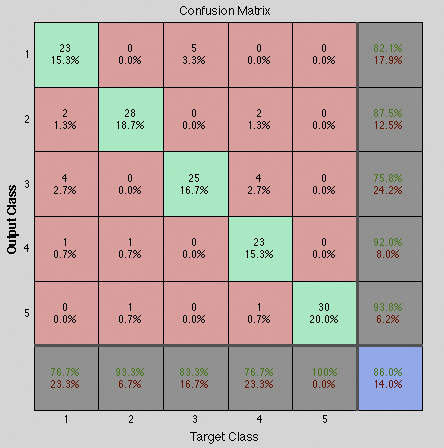
\includegraphics[width=0.4\textwidth]{Table3}
  \caption{Confusion matrix for CENTRIST features. 1-Coast; 2-Forest; 3-Highway; 4-Mountain; 5-Tall Building}
  \label{fig:table3}
\end{figure}

%----------------------------------------------------------------------
% SECTION IV: Color Histogram
%----------------------------------------------------------------------
\section{Color Histogram}
\label{sec:Color}
In scope of scene classification problem, color descriptors cannot be considered reliable for the reason that colors are the matter of constant change. The same scene appears in different colors depending on the time of the day or the season for example.

A lot of papers still offer color descriptors in the combination of texture descriptors and overall experiments show that such combinations improve the performance of classification.

For this project, a simple color histogram descriptor was implemented. The histogram is computed by counting the number of pixels corresponding to the  following colors: red, yellow, green, cyan, blue, magenta, white and black. It is performed first through converting the image to HSV color space and evaluating each plane in order to determine the number of pixels belonging to each of the selected color categories. The number of black and white pixels are estimated through Saturation and Value planes, and the rest of color categories are determined through Hue plane. Every pixel color category is then normalized by dividing the count of the pixels by the number of pixel in the image.
A 8-bin color histogram formats 1x8 feature vector (see figure \ref{fig:image6_7}.b).

\begin{figure}
  \centering
	\mbox{
	\subfigure{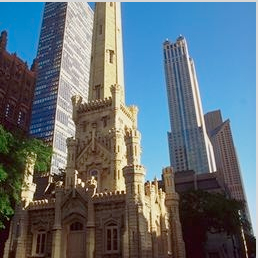
\includegraphics[width=0.2\textwidth]{Image6}
	~
	\subfigure{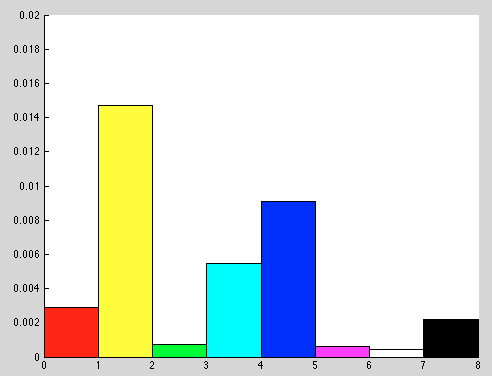
\includegraphics[width=0.25\textwidth]{Image7} }}}
  	\caption{a) Tall Building Image and b) Color Histogram Image Representation}
  	\label{fig:image6_7}
\end{figure}

Classification accuracy for color histogram features was evaluated using MLP Neural Network (8 input, 8 hidden, 5 output neurons) using 150 testing images from five different categories of scenes. Classification error for color histogram descriptor is 50\%, i.e. half of images were misclassified (see figure \ref{fig:table4}). Color histogram features performed the worst for Coast category images (only 13\% accuracy), the best performance is seen for Forest images (83\% accuracy). 
\begin{figure}
  \centering
    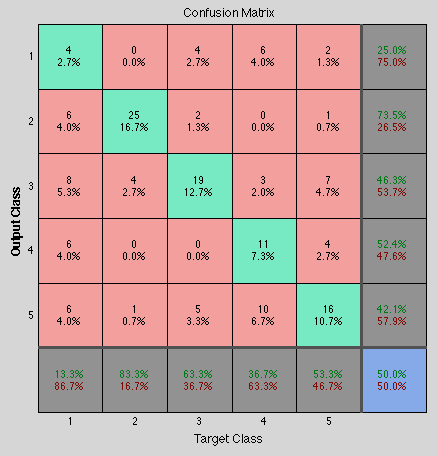
\includegraphics[width=0.4\textwidth]{Table4}
  \caption{Confusion matrix for Color Histogram features. 1-Coast; 2-Forest; 3-Highway; 4-Mountain; 5-Tall Building}
  \label{fig:table4}
\end{figure}
Experiments proved that color cannot be used as a reliable feature for scene categorization problem, but as mentioned before, our study is concerned with improving classification accuracy by adding color features to Gabor-\textsc{Gist} and \textsc{Centrist} features and forming the hybrid feature vector that is expected to provide the minimum misclassification rate.
%----------------------------------------------------------------------
% SECTION V: Combining
%----------------------------------------------------------------------
\section{Hybrid Descriptors}
\label{sec:Hybrid}

\subsection{Method 1: Voting Algorithm}
\label{subsec:Hybrid_Voting}
In order to combine the different feature vectors, a voting algorithm has been coded in the \textsc{Matlab} function \texttt{votingAlgo}. The file \texttt{testVotingAlgoFunction.m} can be used to test the function using Gabor feature vector, Gabor-\textsc{Gist} descriptor and \textsc{Centrist} feature vector, and display the output. It can also run the tests several times and give an average performance. For the voting algorithm, training images are split randomly into a training and a testing set with a chosen percentage. The results for the voting algorithm were not as good as expected. Indeed, figure \ref{fig:votingAlgo} shows that a lot of images are misclassified, knowing that there should be 15 images classified in each category.\\
\begin{figure}
  \centering
    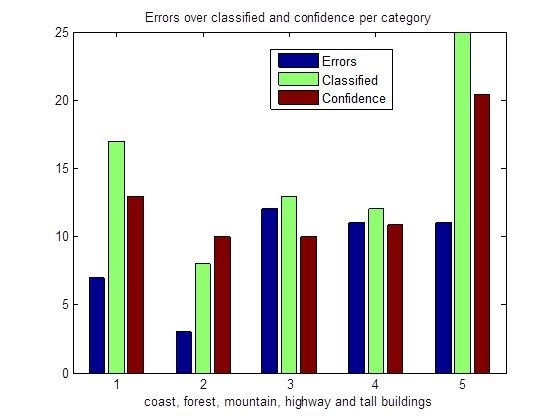
\includegraphics[width=0.5\textwidth]{votingAlgo}
  \caption{Performance for the voting algorithm: results obtained for classification of 15 images of 5 different classes}
  \label{fig:votingAlgo}
\end{figure}
The following of the paper details the classical classifier, the neural network, that has been trained with the feature vectors in order to solve the scene classification problem. 
\subsection{Method 2: Neural Network}
\label{subsec:Hybrid_NN}
The first step that needs to be done in order to create the hybrid feature vector is data scaling. Features extracted with each approach have to be equally weighted. Scaling values of vector $b = [b_{min} , b_{max}]$ in the range of vector $a= [a_{min} , a_{max}]$ values is performed using equation (\ref{eq:rescale}).
\begin{equation}
\label{eq:rescale}
y = (x - b_{min})\frac{a_{max}-a_{min}}{b_{max}-b_{min}}+a_{min}
\end{equation}
 where $x$ is the initial value of vector $b$ and $y$ the rescaled value of $b$ in the range of $a$. 
\begin{figure}
  \centering
    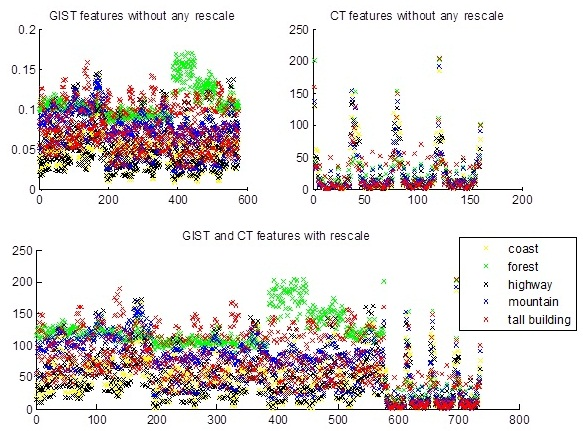
\includegraphics[width=0.5\textwidth]{features}
  \caption{a) Gabor-\textsc{Gist} and \textsc{Centrist} without rescale and  b) Gabor-\textsc{Gist} and \textsc{Centrist} after rescale}
  \label{fig:features}
\end{figure}


Figure \ref{fig:features} shows the effect of applying equation (\ref{eq:rescale}) to Gabor-\textsc{Gist} and \textsc{Centrist} feature vectors. This will later enable the neural network to take them both into account with same weight. \\

In previous stages, input matrices for each descriptor were built and targets stayed the same for the same dataset. In order to create the hybrid vector of features, all that needs to be done is appending one matrix to another ([features1; features2]) and train the MLP network on the new combined input matrix. The same procedure applies for testing input matrix. In the following sub-sections, different combinations of features are analysed and classification accuracy is evaluated.


\subsubsection{Gabor + \textsc{Centrist} Hybrid Results}
\label{subsubsec:resGab_CENTRIST}
The confusion matrix produced by testing the images based on Gabor-\textsc{Gist} and \textsc{Centrist} descriptors is shown in figure \ref{fig:table5}. It indicates potential improvement from combining the features together (if mutual classification compensation occurs). On practice, significant classification error disease occurred, and overall accuracy raised from 86\% (figure \ref{fig:table2}) to 93.3\%(figure \ref{fig:table5}). Features compensated each other deficiencies and didn't create any noticeable confusion. 
\begin{figure}
  \centering
    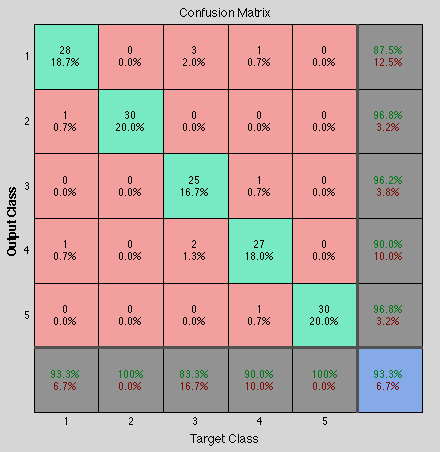
\includegraphics[width=0.4\textwidth]{Table5}
  \caption{Confusion matrix for Gabor + CENTRIST hybrid features. 1-Coast; 2-Forest; 3-Highway; 4-Mountain; 5-Tall Building}
  \label{fig:table5}
\end{figure}
\subsubsection{Gabor + Color Histogram Hybrid Results}
\label{subsubsec:resGab_Color}
Our team was pretty sceptical about combining color histograms with features extracted with other methods, as color histograms performed poorly. The guess was that color histogram features would add more confusion than do any good. However, experiments demonstrated slight performance improvement from 86\% accuracy (Gabor-\textsc{Gist} only) to 89.3\% (Gabor-\textsc{Gist} and color histogram). Gabor-\textsc{Gist} and color histogram hybrid improved the correct classification rate for Coast, Highway and Mountain categories. However, performance decreased for Forest and Tall Building scene classes.

\subsubsection{\textsc{Centrist} + Color Histogram Hybrid Results}
\label{subsubsec:resCENTRIST_Color}
Adding the color histogram descriptor to \textsc{Centrist} also improved the classification accuracy. Improvement occurred for Coast, Forest and Mountain categories but a performance decrease was observed for Highway and Tall Building scene classes. Not that for both Gabor-\textsc{Gist} and \textsc{Centrist}, adding color histogram feature vector improves Coast and Mountain correct classification and reduces Tall building classification. However, the behaviour differs for Highway and Forest images. 

\subsubsection{Gabor + \textsc{Centrist} + Color Histogram Hybrid Results}
\label{subsubsec:resGab_CENTRIST_Color}
\begin{figure}
  \centering
    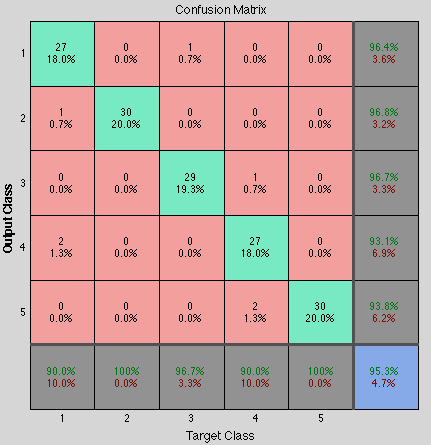
\includegraphics[width=0.4\textwidth]{Table6}
  \caption{Confusion Matrix for Gabor-\textsc{Gist} + \textsc{Centrist} + Color histogram hybrid features. 1-Coast; 2-Forest; 3-Highway; 4-Mountain; 5-Tall Building}
  \label{fig:table6}
\end{figure}
Finally, all the features extracted with the three methods studied in this work (Gabor-\textsc{Gist}, \textsc{Centrist} and color histogram) were combined. As expected, this is the combination that performed the best. Compared to Gabor-\textsc{Gist} + \textsc{Centrist} hybrid, the classification accuracy increased from 93.3\% (figure \ref{fig:table5}) to 95.3\% (figure \ref{fig:table6}). Significant improvement occurred for Highway category (83.3\% category accuracy to 96.6\%), and slight accuracy decrease was demonstrated in Coast category (93.3\% to 90\% class accuracy).


%----------------------------------------------------------------------
% SECTION V: Conclusion
%----------------------------------------------------------------------
\section{Conclusion}
\label{sec:Conclusion}
This paper shows that combining Gabor-\textsc{Gist} descriptor with \textsc{Centrist} and color histogram feature vectors is particularly efficient for scene classification. Indeed, the accuracy obtained using a Neural Network as a classifier is above 95\% for the provided dataset of images. This very high rate of correctly classified images is made possible by the complementarity of the methods used: because Gabor-\textsc{Gist}, \textsc{Centrist} and color histogram have their maximum efficiency for different categories, the overall accuracy is increased when they are combined. \\
Finally, we can say that this combination of three descriptors is very interesting and competitive when compared to other existing methods that can be found in scene classification papers. 

%----------------------------------------------------------------------
\bibliographystyle{ieee} 
\bibliography{ieee} 


\end{document}


